% Options for packages loaded elsewhere
\PassOptionsToPackage{unicode}{hyperref}
\PassOptionsToPackage{hyphens}{url}
%
\documentclass[
]{article}
\usepackage{lmodern}
\usepackage{amssymb,amsmath}
\usepackage{ifxetex,ifluatex}
\ifnum 0\ifxetex 1\fi\ifluatex 1\fi=0 % if pdftex
  \usepackage[T1]{fontenc}
  \usepackage[utf8]{inputenc}
  \usepackage{textcomp} % provide euro and other symbols
\else % if luatex or xetex
  \usepackage{unicode-math}
  \defaultfontfeatures{Scale=MatchLowercase}
  \defaultfontfeatures[\rmfamily]{Ligatures=TeX,Scale=1}
\fi
% Use upquote if available, for straight quotes in verbatim environments
\IfFileExists{upquote.sty}{\usepackage{upquote}}{}
\IfFileExists{microtype.sty}{% use microtype if available
  \usepackage[]{microtype}
  \UseMicrotypeSet[protrusion]{basicmath} % disable protrusion for tt fonts
}{}
\makeatletter
\@ifundefined{KOMAClassName}{% if non-KOMA class
  \IfFileExists{parskip.sty}{%
    \usepackage{parskip}
  }{% else
    \setlength{\parindent}{0pt}
    \setlength{\parskip}{6pt plus 2pt minus 1pt}}
}{% if KOMA class
  \KOMAoptions{parskip=half}}
\makeatother
\usepackage{xcolor}
\IfFileExists{xurl.sty}{\usepackage{xurl}}{} % add URL line breaks if available
\IfFileExists{bookmark.sty}{\usepackage{bookmark}}{\usepackage{hyperref}}
\hypersetup{
  hidelinks,
  pdfcreator={LaTeX via pandoc}}
\urlstyle{same} % disable monospaced font for URLs
\usepackage{longtable,booktabs}
% Correct order of tables after \paragraph or \subparagraph
\usepackage{etoolbox}
\makeatletter
\patchcmd\longtable{\par}{\if@noskipsec\mbox{}\fi\par}{}{}
\makeatother
% Allow footnotes in longtable head/foot
\IfFileExists{footnotehyper.sty}{\usepackage{footnotehyper}}{\usepackage{footnote}}
\makesavenoteenv{longtable}
\usepackage{graphicx}
\makeatletter
\def\maxwidth{\ifdim\Gin@nat@width>\linewidth\linewidth\else\Gin@nat@width\fi}
\def\maxheight{\ifdim\Gin@nat@height>\textheight\textheight\else\Gin@nat@height\fi}
\makeatother
% Scale images if necessary, so that they will not overflow the page
% margins by default, and it is still possible to overwrite the defaults
% using explicit options in \includegraphics[width, height, ...]{}
\setkeys{Gin}{width=\maxwidth,height=\maxheight,keepaspectratio}
% Set default figure placement to htbp
\makeatletter
\def\fps@figure{htbp}
\makeatother
\setlength{\emergencystretch}{3em} % prevent overfull lines
\providecommand{\tightlist}{%
  \setlength{\itemsep}{0pt}\setlength{\parskip}{0pt}}
\setcounter{secnumdepth}{-\maxdimen} % remove section numbering

\author{}
\date{}

\begin{document}

\hypertarget{header-n0}{%
\section{软件学院书籍影视交流平台------需求规格说明书}\label{header-n0}}

\hypertarget{header-n1369}{%
\subsection{引言}\label{header-n1369}}

a

\hypertarget{header-n1371}{%
\subsection{摘要}\label{header-n1371}}

a

\hypertarget{header-n1374}{%
\subsection{概述}\label{header-n1374}}

\hypertarget{header-n3}{%
\subsubsection{用户简介}\label{header-n3}}

本项目所针对的用户主要以在校大学生以及课程负责人,首先是因为环境方面,我们处于大学,仍在经营学业,无法过多宣传本项目,只能通过同学间的互相帮助来完成项目的各方面;其次是本项目是作为课程的一个任务,在提交时,对本项目进行查验的是课程的负责人。因此,本项目的用户大致分为这两类。当然如果存在其他用户,本项目也能为其提供很好的使用体验。

\hypertarget{header-n5}{%
\subsubsection{项目的目的与目标}\label{header-n5}}

本项目的目的和目标是为了能给对书籍、影视等艺术作品感兴趣的用户提供一个交流的平台,从而让思想在这里碰撞,让用户能够随心所欲的发表自己的观点,以及与其他用户进行讨论。本项目希望能够为大家搭建一个更加自由的平台,每个人的评论能够被其他人看到并且可以对其他人的观点进行评价,让用户们都能在这里找到自己喜爱的书籍影视作品,以及分享自己所喜爱的书籍影视作品。

\hypertarget{header-n7}{%
\subsubsection{涉及名词解释}\label{header-n7}}

{[}1{]}
用户:包含游客以及已经完成注册的用户,在平台中主要进行交互的对象。

{[}2{]}
小组管理员:指在参与小组中的一个负责的对象,能够对其小组的帖子进行管理。

{[}3{]} 系统管理员:指整个平台的管理员,与实际平台的功能等等关联不大。

\hypertarget{header-n11}{%
\subsubsection{参考资料}\label{header-n11}}

{[}1{]} 吕云翔.软件工程实用教程{[}M{]}.北京:清华大学出版社,2015.

\hypertarget{header-n13}{%
\subsubsection{相关文档}\label{header-n13}}

{[}1{]} 《软件开发企划书》

{[}2{]} 《软件设计说明书》

{[}3{]} 《部署文档》

{[}4{]} 《测试报告》

{[}5{]} 《用户使用说明书》

\hypertarget{header-n19}{%
\subsubsection{版本更新信息}\label{header-n19}}

@版本更新记录表

\begin{longtable}[]{@{}ccccc@{}}
\toprule
版本 & 更新者 & 更新 & 更新纪要 & 完成度\tabularnewline
\midrule
\endhead
v1.0.0 & 杨壮 & 2020.4.19 & 项目创建 & 暂无\tabularnewline
v1.0.1 & 张涵珂 & 2020.4.22 & 概述、系统总体简介 & 暂无\tabularnewline
v1.0.2 & 杨哲宇 & 2020.4.26 & 系统功能需求-同理图形式分析 &
暂无\tabularnewline
v1.0.3 & 叶天宇 & 2020.4.26 & 接口与需求 & 暂无\tabularnewline
& & & &\tabularnewline
& & & &\tabularnewline
& & & &\tabularnewline
\bottomrule
\end{longtable}

\hypertarget{header-n70}{%
\subsection{系统总体简介}\label{header-n70}}

\hypertarget{header-n71}{%
\subsubsection{角色定义}\label{header-n71}}

\begin{longtable}[]{@{}cc@{}}
\toprule
角色名称 & 角色定义及说明\tabularnewline
\midrule
\endhead
游客 &
对平台的内容、其他用户的帖子具有读权限,可以进行浏览,无法加入小组、无法发帖,也无法对其他帖子进行评论或者举报。\tabularnewline
注册用户 &
具有使用平台的权限,可以发帖、评论、举报,可以加入讨论小组,可以使用平台的几乎所有功能\tabularnewline
小组管理员 &
指某小组的管理人员,可以对本小组发布的帖子进行删除或者屏蔽,以及对本小组的用户进行剔除或者转让小组管理员。\tabularnewline
审查员 &
对小组管理员进行审查的人员,对滥用职权的小组管理员进行警告、撤职、封号等。\tabularnewline
系统管理员 &
整个平台的管理员,具有全局管理用户发布的帖子的权限,以及处理用户举报的不合法帖子,对被举报的帖子进行相应的处罚措施。\tabularnewline
开发人员 &
整个平台的开发人员,负责平台的开发,对用户的一些需求进行解决,定期对平台进行更新,以及对用户的数据进行安全保存。\tabularnewline
\bottomrule
\end{longtable}

\hypertarget{header-n94}{%
\subsubsection{系统的开发运行环境}\label{header-n94}}

使用Windows系统进行开发,开发环境如下:

\begin{verbatim}
操作系统:Windows 10
数据库系统:MySQL
IDE:Visual Studio Code
测试工具:Google Chrome
编码方式:UTF-8
\end{verbatim}

\textbf{运行环境如下:}

\begin{verbatim}
操作系统:Windows、Android
运行界面:WEB
\end{verbatim}

\hypertarget{header-n99}{%
\subsubsection{工作流程}\label{header-n99}}

网站的总体工作图如下:

\begin{figure}
\centering
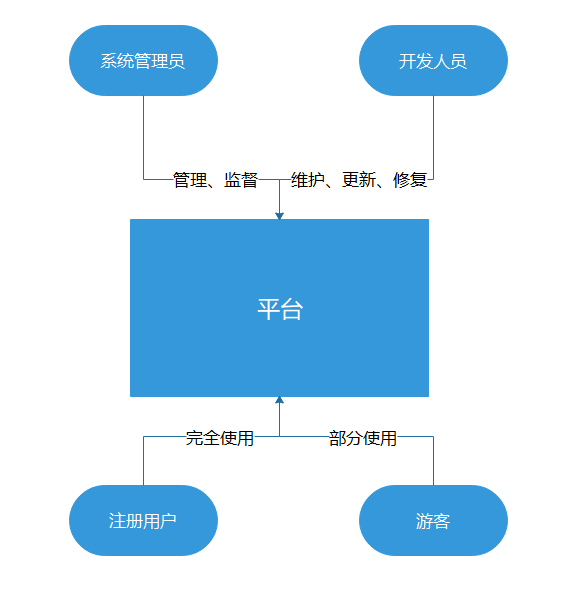
\includegraphics{D:/code/buaase-2020-chatplatform/docs/生成的LaTeX/pic/1.PNG}
\caption{}
\end{figure}

本项目的工作流程主要分为五大方面,网站的总体工作流程图如下所示。

首先是项目启动,小组各人员进行成员分工,确定各自负责的板块,然后开始着手项目分析,确定本项目的各个模块的细节信息,然后开始项目前后端设计,设计如何进行编写源代码,然后进行项目全面开发,开始动工编写代码,前端和后端分别进行并定期交流以实现前后端更好的交互。在编写完成后对项目功能进行相应的测试,进行项目的改进,最后完成项目。具体可以参考附件甘特图。

\begin{figure}
\centering
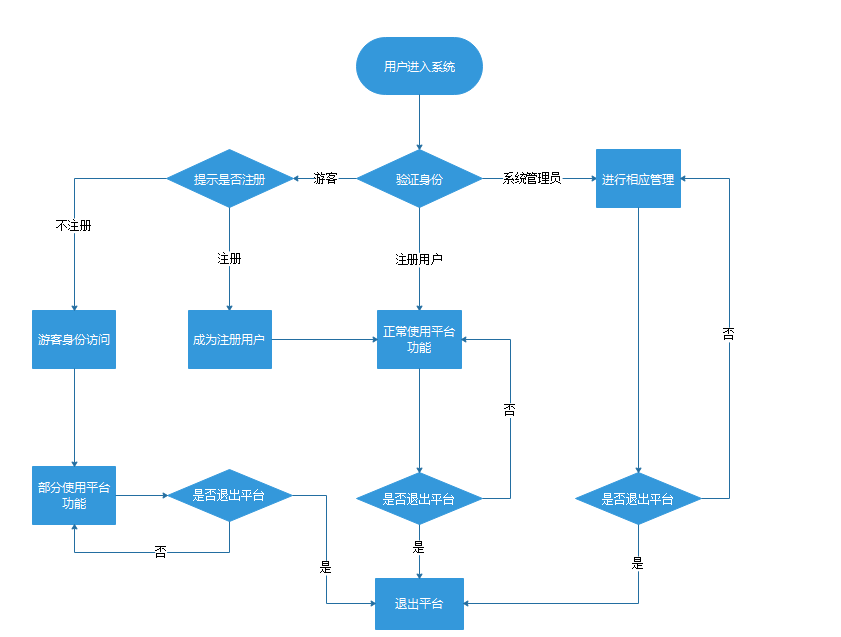
\includegraphics{D:/code/buaase-2020-chatplatform/docs/生成的LaTeX/pic/2.PNG}
\caption{}
\end{figure}

\hypertarget{header-n105}{%
\subsubsection{系统的未来拓展}\label{header-n105}}

本项目的初衷是为了搭建一个书籍影视的交流平台,在未来拓展方面,本项目可以增加其他类型的板块,例如书法、美术作品,增设不同类型的模块,不仅限于书籍和影视,从用户的兴趣入手,增添各类模块,让用户在这个平台上能够找到自己的所有爱好,每个爱好都能发表自己的观点。

另外的方面就是对平台的适应性进行调整,可以开发跨平台APP。让这款平台能够更好的符合用户的使用标准,不再局限于某一方面。然后再就是与其他的软件或者其他平台实现交互,让其他平台的用户也能够觉得轻松的在本平台上交流,而不再局限于单方面。

\hypertarget{header-n108}{%
\subsection{系统功能需求}\label{header-n108}}

\hypertarget{header-n109}{%
\subsubsection{功能模块总体设计}\label{header-n109}}

\begin{figure}
\centering
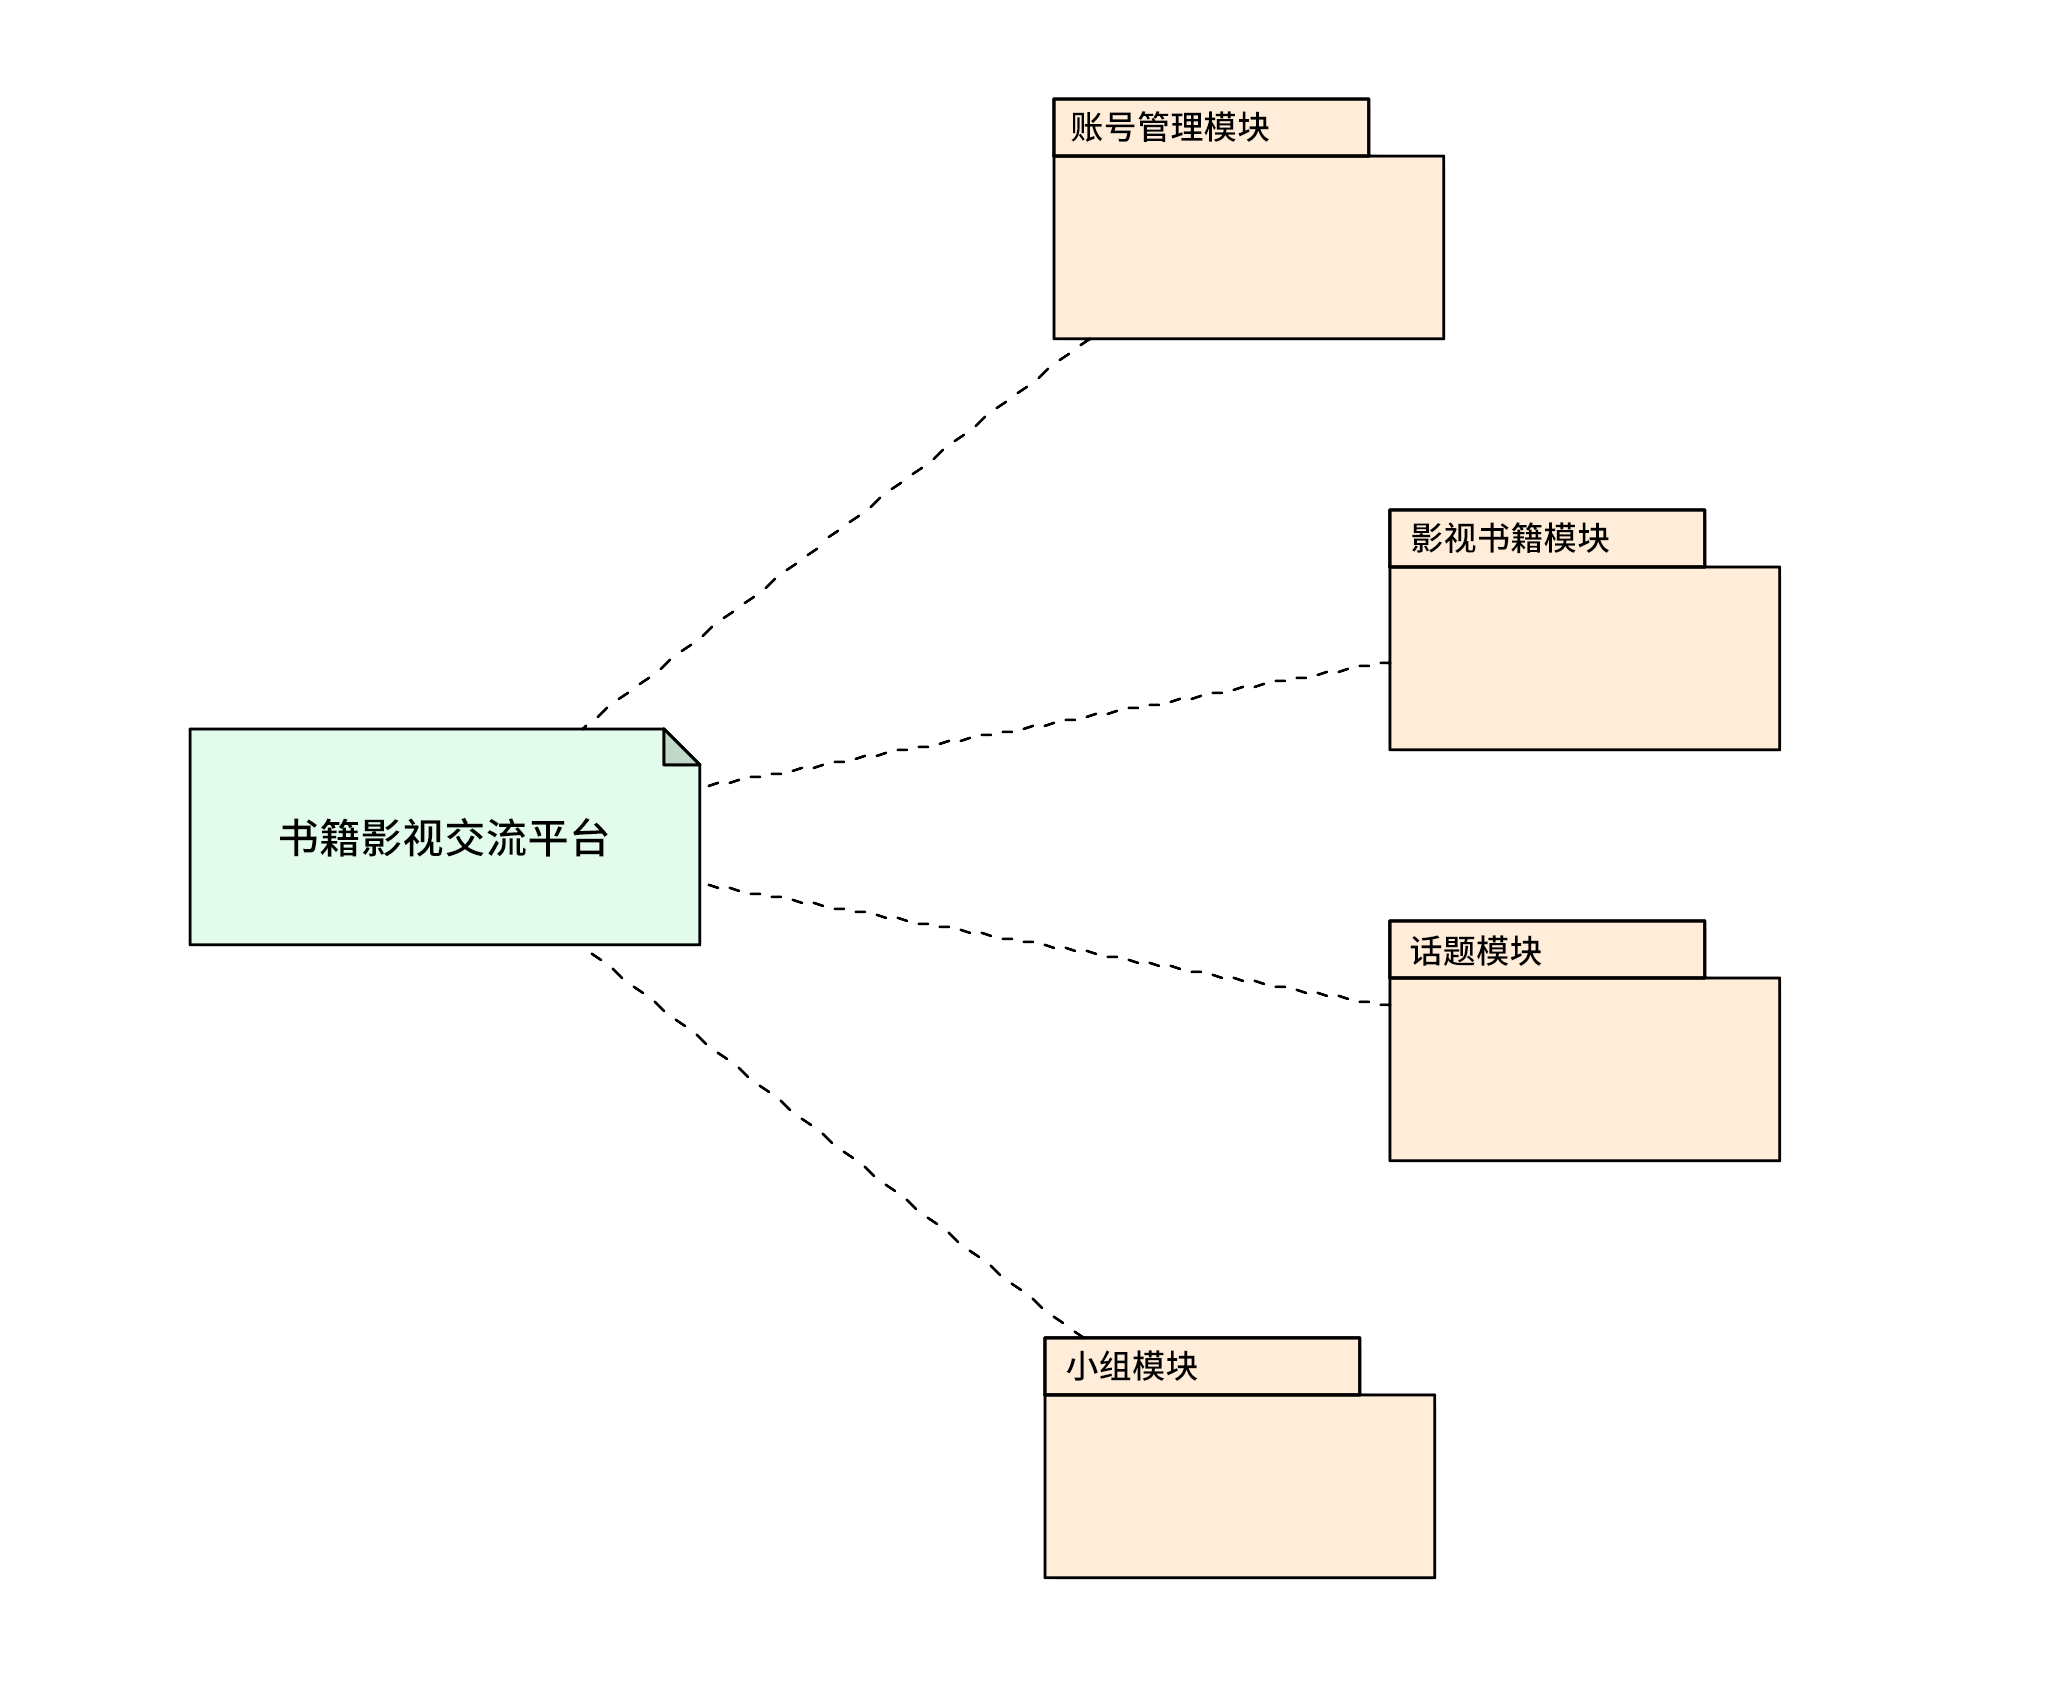
\includegraphics{D:/code/buaase-2020-chatplatform/docs/生成的LaTeX/pic/ModuleDesign.png}
\caption{}
\end{figure}

\hypertarget{header-n111}{%
\subsubsection{用例图形式分析}\label{header-n111}}

\hypertarget{header-n112}{%
\paragraph{账号管理模块}\label{header-n112}}

用例图如图所示

\begin{figure}
\centering
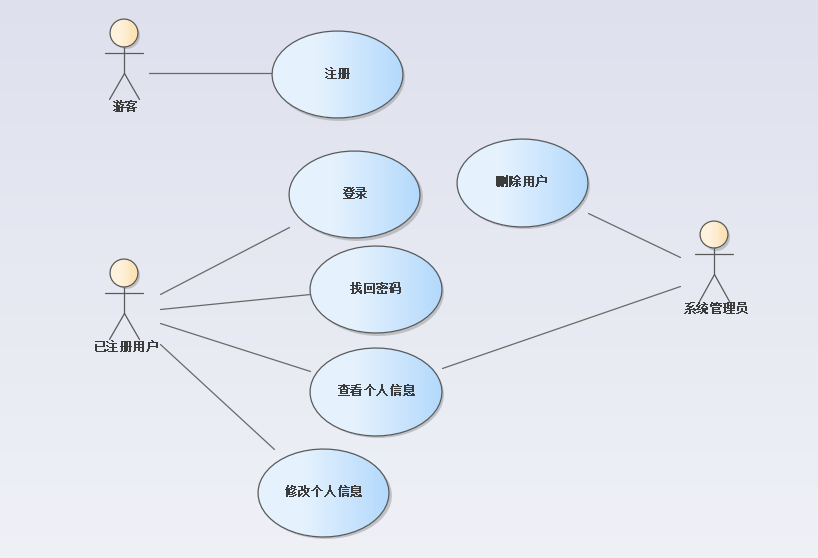
\includegraphics{D:/code/buaase-2020-chatplatform/docs/生成的LaTeX/pic/zhanghaoyl.png}
\caption{}
\end{figure}

以下为用例表

\begin{longtable}[]{@{}llll@{}}
\toprule
编号 & 101 & 用例名称 & 注册\tabularnewline
\midrule
\endhead
使用人员 & 游客 & 扩展点 & 无\tabularnewline
输入 & 用户注册时的基本信息 & &\tabularnewline
系统响应 & 系统将用户注册时的信息保存在数据库中 & &\tabularnewline
输出 & 用户可以用注册的用户名及密码进行登陆操作 & &\tabularnewline
前置条件 & 未注册用户申请注册 & 后置条件 &
注册成功,成为会员\tabularnewline
活动步骤 & 1. 未注册用户选择注册 \textless br /\textgreater{}2.
系统返回一个注册页面 \textless br /\textgreater{}3.
未注册用户输入相关注册信息 \textless br /\textgreater{}4.
系统验证输入成功 \textless br /\textgreater{}5. 用户提交注册信息
\textless br /\textgreater{}6. 系统提交注册成功并返回首页 &
&\tabularnewline
异常处理 & 1. 注册时输入信息和系统验证不一致系统给出提示\textless br
/\textgreater{}2. 用户名已注册,系统给出提示然后并返回注册界面
\textless br /\textgreater{}3. 系统异常,无法注册,并给出相应信息。 &
&\tabularnewline
\bottomrule
\end{longtable}

\begin{longtable}[]{@{}llll@{}}
\toprule
编号 & 102 & 用例名称 & 登录\tabularnewline
\midrule
\endhead
使用人员 & 已注册用户 & 扩展点 & 无\tabularnewline
输入 & 注册时的用户名和密码 & &\tabularnewline
系统响应 & 用户的登陆时间、次数等存入数据库,并保存登录状态 &
&\tabularnewline
输出 & 用户登录获得的tokens & &\tabularnewline
前置条件 & 该用户必须是本站已注册成功用户 & 后置条件 &
该用户登录成功\tabularnewline
活动步骤 & 1. 该会员点击登录\textless br /\textgreater{}2.
系统返回登录页面\textless br /\textgreater{}3.
用户输入用户名、密码及验证码并提交\textless br /\textgreater{}4.
系统进行验证,验证成功,记录该用户的登录状态并跳转到主界面 &
&\tabularnewline
异常处理 & 1.
用户忘记密码,选择``找回密码''功能,进入找回密码用例\textless br
/\textgreater{}2. 系统验证用户登录信息有误,提示重新登录\textless br
/\textgreater{}3. 系统处理异常,给出相应的错误信息 & &\tabularnewline
\bottomrule
\end{longtable}

\begin{longtable}[]{@{}llll@{}}
\toprule
编号 & 103 & 用例名称 & 找回密码\tabularnewline
\midrule
\endhead
使用人员 & 已注册用户 & 扩展点 & 无\tabularnewline
输入 & 用户注册时的邮箱或密码提示问题 & &\tabularnewline
系统响应 &
系统根据注册邮箱账号或密码提示问题找到相应的用户并返回起对应的
密码设置主页 & &\tabularnewline
输出 & 用户重置自己的密码 & &\tabularnewline
前置条件 & 该用户必须是本站已注册成功用户 & 后置条件 &
系统返回设置密码的页面让用户重置密码\tabularnewline
活动步骤 & 1. 用户选择``找回密码'' \textless br /\textgreater{}2.
系统返回一个找回密码页面(要求用户输入注册时的邮箱号,并回答
对提示问题,系统会自动向邮箱中设发送注册的密码) \textless br
/\textgreater{}3. 用户输入邮箱中的密码并填写提交 4.
系统进行验证,成功后,跳转到个人主界面 & &\tabularnewline
异常处理 & 1.
若用户在步骤中输入邮箱或提示问题错误,系统会给出提示。\textless br
/\textgreater{}2. 系统处理异常,系统给出相应的提示信息 &
&\tabularnewline
\bottomrule
\end{longtable}

\begin{longtable}[]{@{}llll@{}}
\toprule
编号 & 104 & 用例名称 & 查看个人信息\tabularnewline
\midrule
\endhead
使用人员 & 已注册用户、管理员 & 扩展点 & 无\tabularnewline
输入 & 点击相关的查看信息按钮 & &\tabularnewline
系统响应 & 系统根据需要查看的用户,从数据库中查询读取信息 &
&\tabularnewline
输出 & 系统显示用户的个人信息 & &\tabularnewline
前置条件 & 用户必须是本系统的成功 注册用户或者管理员 & 后置条件 &
系统显示个人信息页面\tabularnewline
活动步骤 & 1. 用户选择``查看个人信息'' \textless br /\textgreater{}2.
系统显示相应的个人信息 & &\tabularnewline
异常处理 & 系统处理异常,系统给出相应的提示信息 & &\tabularnewline
\bottomrule
\end{longtable}

\begin{longtable}[]{@{}llll@{}}
\toprule
编号 & 105 & 用例名称 & 修改个人信息\tabularnewline
\midrule
\endhead
使用人员 & 已注册用户 & 扩展点 & 无\tabularnewline
输入 & 用户输入个人的相关信息 & &\tabularnewline
系统响应 & 系统在数据库中用户现在的个人信息替换以前的个人信息 &
&\tabularnewline
输出 & 修改是否成功的提示信息 & &\tabularnewline
前置条件 & 用户已经是此系统的注册 用户且已经登录 & 后置条件 &
该用户修改个人信息成功\tabularnewline
活动步骤 & 1. 用户选择``修改信息 \textless br /\textgreater{}2.
系统返回修改信息界面 \textless br /\textgreater{}3. 用户修改信息并提交
\textless br /\textgreater{}4. 系统进行系统验证,验证成功后提示修改成功
& &\tabularnewline
异常处理 & 1. 系统验证输入信息有误,提示重新输入 \textless br
/\textgreater{}2. 系统处理异常,系统给出相应的提示信息 &
&\tabularnewline
\bottomrule
\end{longtable}

\begin{longtable}[]{@{}llll@{}}
\toprule
编号 & 106 & 用例名称 & 删除用户\tabularnewline
\midrule
\endhead
使用人员 & 管理员 & 扩展点 & 无\tabularnewline
输入 & 需要删除的用户ID & &\tabularnewline
系统响应 & 系统删除数据库中相应的用户信息 & &\tabularnewline
输出 & 删除是否成功的提示 & &\tabularnewline
前置条件 & 用户是管理员并且处于用户列表页面 & 后置条件 &
删除用户成功\tabularnewline
活动步骤 & 1. 管理员选择需要删除的用户并点击删除选项\textless br
/\textgreater{}2. 系统提示管理员将要删除该用户并得到用户的确认
\textless br /\textgreater{}3. 系统提示删除用户成功并返回用户列表页面 &
&\tabularnewline
异常处理 & 系统异常,并给出相应的提示信息 & &\tabularnewline
\bottomrule
\end{longtable}

\hypertarget{header-n362}{%
\paragraph{影视书籍模块}\label{header-n362}}

用例图如图所示

\begin{figure}
\centering
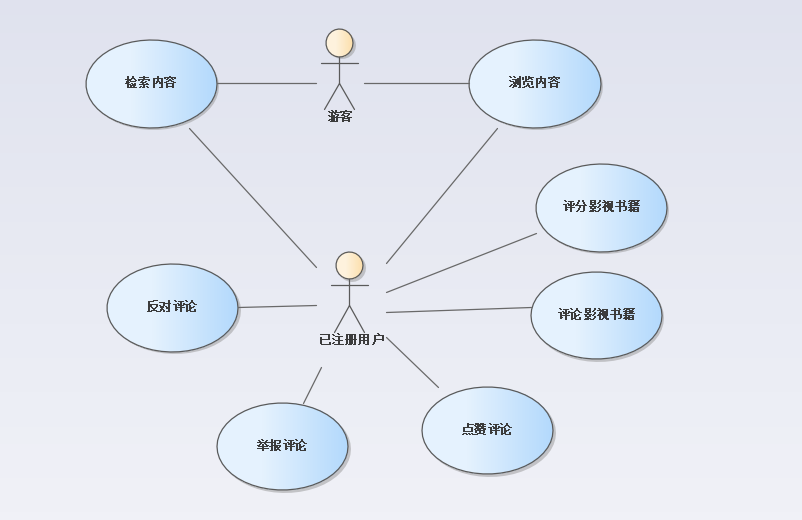
\includegraphics{D:/code/buaase-2020-chatplatform/docs/生成的LaTeX/pic/yingshishujiyl.png}
\caption{}
\end{figure}

\begin{longtable}[]{@{}llll@{}}
\toprule
编号 & 201 & 用例名称 & 浏览内容\tabularnewline
\midrule
\endhead
使用人员 & 游客,已注册用户 & 扩展点 & 无\tabularnewline
输入 & 想要浏览的页面 & &\tabularnewline
系统响应 & 加载相应的内容 & &\tabularnewline
输出 & 显示页面 & &\tabularnewline
前置条件 & 用户处于相应的页面 & 后置条件 & 成功加载页面\tabularnewline
活动步骤 & 1.用户点击想要浏览的内容\textless br
/\textgreater{}2.用户查看内容 & &\tabularnewline
异常处理 & 用户想要查看内容不存在,系统给出相应的提示 & &\tabularnewline
\bottomrule
\end{longtable}

\begin{longtable}[]{@{}llll@{}}
\toprule
编号 & 202 & 用例名称 & 检索内容\tabularnewline
\midrule
\endhead
使用人员 & 游客,已注册用户 & 扩展点 &
用户可以根据检索得到的内容进行浏览\tabularnewline
输入 & 检索关键词 & &\tabularnewline
系统响应 & 根据关键词在数据库中查询内容 & &\tabularnewline
输出 & 符合关键词的内容 & &\tabularnewline
前置条件 & 用户处于可以检索的主题 & 后置条件 &
成功加载页面\tabularnewline
活动步骤 & 1.用户点击检索栏\textless br
/\textgreater{}2.用户输入关键词\textless br
/\textgreater{}3.用户点击检索按钮\textless br
/\textgreater{}4.系统给出检索结构 & &\tabularnewline
异常处理 & 关键词包含敏感词,系统不返回结果 & &\tabularnewline
\bottomrule
\end{longtable}

\begin{longtable}[]{@{}llll@{}}
\toprule
编号 & 203 & 用例名称 & 评论影视书籍\tabularnewline
\midrule
\endhead
使用人员 & 已注册用户 & 扩展点 &\tabularnewline
输入 & 评论标题,评论内容 & &\tabularnewline
系统响应 & 判断评论是否符合要求,若符合,则进行上传,发布 &
&\tabularnewline
输出 & 评论是否成功的提示 & &\tabularnewline
前置条件 & 用户处于书籍或影视条目页面,且已登录 & 后置条件 &
用户评论成功\tabularnewline
活动步骤 & 1.用户进入一个影视/书籍条目\textless br
/\textgreater{}2.用户点击评论按钮\textless br
/\textgreater{}3.用户输入评论标题和评论内容\textless br
/\textgreater{}4.用户从一星到五星中选择一个按钮点击\textless br
/\textgreater{}5.用户点击确认按钮\textless br
/\textgreater{}6.系统给出发表成功与否的提示 & &\tabularnewline
异常处理 & 1.评论格式不符合要求,系统给出提示\textless br
/\textgreater{}2.用户不是注册用户,或者注册后未登录,系统提示注册/登录 &
&\tabularnewline
\bottomrule
\end{longtable}

\begin{longtable}[]{@{}llll@{}}
\toprule
编号 & 204 & 用例名称 & 评分影视书籍\tabularnewline
\midrule
\endhead
使用人员 & 已注册用户 & 扩展点 &\tabularnewline
输入 & 用户点击的分数(1-5颗星) & &\tabularnewline
系统响应 & 将评分上传数据库 & &\tabularnewline
输出 & 评分成功的提示 & &\tabularnewline
前置条件 & 用户处于书籍或影视条目页面,且已登录 & 后置条件 &
用户评分成功\tabularnewline
活动步骤 & 1.用户进入一个影视/书籍条目\textless br
/\textgreater{}2.用户点击评分按钮\textless br
/\textgreater{}3.用户从一星到五星中选择一个按钮点击 \textless br
/\textgreater{}4.用户点击确认按钮 \textless br
/\textgreater{}5.系统给出评分成功与否的提示 & &\tabularnewline
异常处理 & 用户不是注册用户,或者注册后未登录,系统提示注册/登录 &
&\tabularnewline
\bottomrule
\end{longtable}

\begin{longtable}[]{@{}llll@{}}
\toprule
编号 & 205 & 用例名称 & 点赞评论\tabularnewline
\midrule
\endhead
使用人员 & 已注册用户 & 扩展点 &\tabularnewline
输入 & 用户点击 & &\tabularnewline
系统响应 & 点赞数据上传数据库 & &\tabularnewline
输出 & 点赞成功提示 & &\tabularnewline
前置条件 & 用户处于书籍或影视条目的评论列表,且已登录 & 后置条件 &
点赞评论成功\tabularnewline
活动步骤 & 1.用户进入一条评论页面 \textless br
/\textgreater{}2.用户点击点赞按钮 \textless br
/\textgreater{}3.系统给出点赞成功与否的提示 & &\tabularnewline
异常处理 & 用户不是注册用户,或者注册后未登录,系统提示注册/登录 &
&\tabularnewline
\bottomrule
\end{longtable}

\begin{longtable}[]{@{}llll@{}}
\toprule
编号 & 206 & 用例名称 & 反对评论\tabularnewline
\midrule
\endhead
使用人员 & 已注册用户 & 扩展点 &\tabularnewline
输入 & 用户点击 & &\tabularnewline
系统响应 & 反对数据上传数据库 & &\tabularnewline
输出 & 反对成功提示 & &\tabularnewline
前置条件 & 用户处于书籍或影视条目的评论列表,且已登录 & 后置条件 &
反对评论成功\tabularnewline
活动步骤 & 1.用户进入一条评论页面 \textless br
/\textgreater{}2.用户点击反对按钮 \textless br
/\textgreater{}3.系统给出反对成功与否的提示 & &\tabularnewline
异常处理 & 用户不是注册用户,或者注册后未登录,系统提示注册/登录 &
&\tabularnewline
\bottomrule
\end{longtable}

\begin{longtable}[]{@{}llll@{}}
\toprule
编号 & 207 & 用例名称 & 举报评论\tabularnewline
\midrule
\endhead
使用人员 & 已注册用户 & 扩展点 &\tabularnewline
输入 & 用户点击举报按钮,输入举报标题和原因 & &\tabularnewline
系统响应 & 系统判断是否符合要求,若符合,则上传到数据库 &
&\tabularnewline
输出 & 举报成功提交提示 & &\tabularnewline
前置条件 & 用户处于书籍或影视条目的评论列表,且已登录 & 后置条件 &
举报成功提交\tabularnewline
活动步骤 & 1.用户进入一条评论页面 \textless br
/\textgreater{}2.用户点击举报按钮\textless br
/\textgreater{}3.用户输入举报标题和举报内容\textless br
/\textgreater{}4.用户点击提交按钮\textless br
/\textgreater{}5.系统给出提交成功与否的提示 & &\tabularnewline
异常处理 & 1.用户是游客,或者注册后未登录,系统提示注册/登录\textless br
/\textgreater{}2.举报格式不符合要求,系统进行相关提示。 &
&\tabularnewline
\bottomrule
\end{longtable}

\hypertarget{header-n652}{%
\paragraph{话题模块}\label{header-n652}}

用例图如图所示

\begin{figure}
\centering
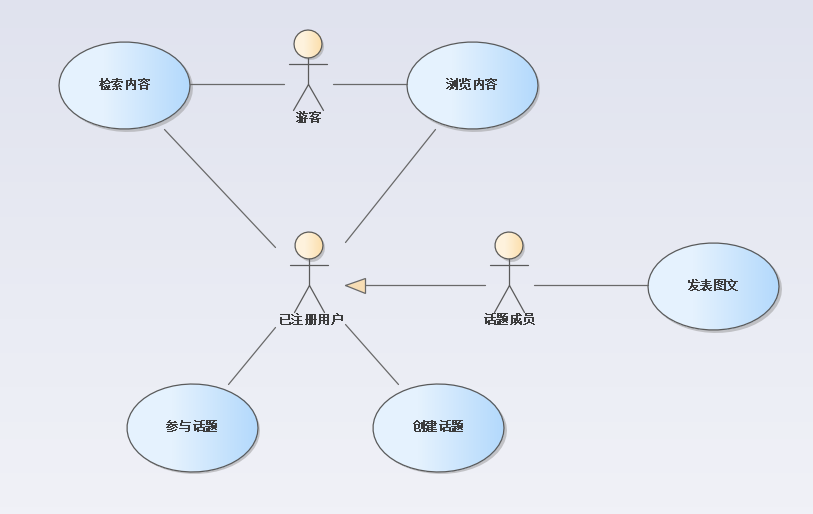
\includegraphics{D:/code/buaase-2020-chatplatform/docs/生成的LaTeX/pic/huatiyl.png}
\caption{}
\end{figure}

\begin{longtable}[]{@{}llll@{}}
\toprule
编号 & 301 & 用例名称 & 浏览内容\tabularnewline
\midrule
\endhead
使用人员 & 游客,已注册用户 & 扩展点 & 无\tabularnewline
输入 & 想要浏览的页面 & &\tabularnewline
系统响应 & 加载相应的内容 & &\tabularnewline
输出 & 显示页面 & &\tabularnewline
前置条件 & 用户处于相应的页面 & 后置条件 & 成功加载页面\tabularnewline
活动步骤 & 1.用户点击想要浏览的内容\textless br
/\textgreater{}2.用户查看内容 & &\tabularnewline
异常处理 & 用户想要查看内容不存在,系统给出相应的提示 & &\tabularnewline
\bottomrule
\end{longtable}

\begin{longtable}[]{@{}llll@{}}
\toprule
编号 & 302 & 用例名称 & 检索内容\tabularnewline
\midrule
\endhead
使用人员 & 游客,已注册用户 & 扩展点 &
用户可以通过检索得到的内容浏览\tabularnewline
输入 & 检索关键词 & &\tabularnewline
系统响应 & 根据关键词在数据库中查询内容 & &\tabularnewline
输出 & 符合关键词的内容 & &\tabularnewline
前置条件 & 用户处于可以检索的主题 & 后置条件 &
成功加载页面\tabularnewline
活动步骤 & 1.用户点击检索栏\textless br
/\textgreater{}2.用户输入关键词\textless br
/\textgreater{}3.用户点击检索按钮\textless br
/\textgreater{}4.系统给出检索结构 & &\tabularnewline
异常处理 & 关键词包含敏感词,系统不返回结果 & &\tabularnewline
\bottomrule
\end{longtable}

\begin{longtable}[]{@{}llll@{}}
\toprule
编号 & 303 & 用例名称 & 参与话题\tabularnewline
\midrule
\endhead
使用人员 & 已注册用户 & 扩展点 &\tabularnewline
输入 & 用户点击 & &\tabularnewline
系统响应 & 系统将该用户标记为该话题参与者上传数据库 & &\tabularnewline
输出 & 参与成功与否的提示 & &\tabularnewline
前置条件 & 用户处于话题页面,且已登录 & 后置条件 &
参与话题成功\tabularnewline
活动步骤 & 1.用户选择一个话题\textless br
/\textgreater{}2.用户点击参与话题\textless br
/\textgreater{}3.系统返回参与是否成功的提示 & &\tabularnewline
异常处理 & 1.用户是游客,或者注册后未登录,系统提示注册/登录 &
&\tabularnewline
\bottomrule
\end{longtable}

\begin{longtable}[]{@{}llll@{}}
\toprule
编号 & 304 & 用例名称 & 创建话题\tabularnewline
\midrule
\endhead
使用人员 & 已注册用户 & 扩展点 &\tabularnewline
输入 & 用户点击,话题相关信息 & &\tabularnewline
系统响应 & 系统判断相关信息受否符合要求,然后将话题上传、发布。 &
&\tabularnewline
输出 & 创建是否成功的提示。 & &\tabularnewline
前置条件 & 用户处于话题页面,且已登录 & 后置条件 &
创建话题成功\tabularnewline
活动步骤 & 1.用户点击创建话题\textless br
/\textgreater{}2.用户输入话题信息\textless br
/\textgreater{}3.用户点击创建按钮\textless br
/\textgreater{}4.系统判断是否符合要求,返回提示 & &\tabularnewline
异常处理 & 1.用户是游客,或者注册后未登录,系统提示注册/登录\textless br
/\textgreater{}2.用户提交的信息不符合要求,系统给出修改意见 &
&\tabularnewline
\bottomrule
\end{longtable}

\begin{longtable}[]{@{}llll@{}}
\toprule
编号 & 305 & 用例名称 & 发表图文\tabularnewline
\midrule
\endhead
使用人员 & 话题成员 & 扩展点 &\tabularnewline
输入 & 用户输入的图片和文字 & &\tabularnewline
系统响应 & 将相关信息上传数据库 & &\tabularnewline
输出 & 发表成功与否的提示 & &\tabularnewline
前置条件 & 用户处于某一话题条目页面,且已登录 & 后置条件 &
发表图文成功\tabularnewline
活动步骤 & 1.用户输入文字,上传图片\textless br
/\textgreater{}2.用户点击发布按钮\textless br
/\textgreater{}3.系统返回参与是否成功的提示 & &\tabularnewline
异常处理 & 1.用户未参与话题,系统提示参与话题。\textless br
/\textgreater{}2.用户发布的图文不合规范,系统提示修改 & &\tabularnewline
\bottomrule
\end{longtable}

\hypertarget{header-n860}{%
\paragraph{小组模块}\label{header-n860}}

用例图如图所示

\begin{figure}
\centering
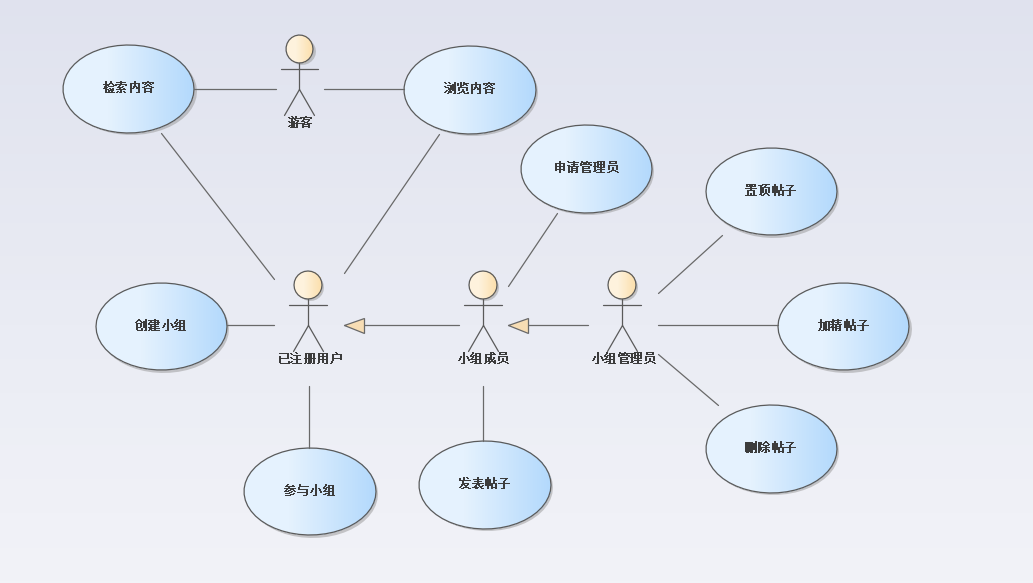
\includegraphics{D:/code/buaase-2020-chatplatform/docs/生成的LaTeX/pic/xiaozuyl.png}
\caption{}
\end{figure}

\begin{longtable}[]{@{}llll@{}}
\toprule
编号 & 401 & 用例名称 & 浏览内容\tabularnewline
\midrule
\endhead
使用人员 & 游客,已注册用户 & 扩展点 & 无\tabularnewline
输入 & 想要浏览的页面 & &\tabularnewline
系统响应 & 加载相应的内容 & &\tabularnewline
输出 & 显示页面 & &\tabularnewline
前置条件 & 用户处于相应的页面 & 后置条件 & 成功加载页面\tabularnewline
活动步骤 & 1.用户点击想要浏览的内容\textless br
/\textgreater{}2.用户查看内容 & &\tabularnewline
异常处理 & 用户想要查看内容不存在,系统给出相应的提示 & &\tabularnewline
\bottomrule
\end{longtable}

\begin{longtable}[]{@{}llll@{}}
\toprule
编号 & 402 & 用例名称 & 检索内容\tabularnewline
\midrule
\endhead
使用人员 & 游客,已注册用户 & 扩展点 &
用户可以通过检索得到的内容浏览\tabularnewline
输入 & 检索关键词 & &\tabularnewline
系统响应 & 根据关键词在数据库中查询内容 & &\tabularnewline
输出 & 符合关键词的内容 & &\tabularnewline
前置条件 & 用户处于可以检索的主题 & 后置条件 &
成功加载页面\tabularnewline
活动步骤 & 1.用户点击检索栏\textless br
/\textgreater{}2.用户输入关键词\textless br
/\textgreater{}3.用户点击检索按钮\textless br
/\textgreater{}4.系统给出检索结构 & &\tabularnewline
异常处理 & 关键词包含敏感词,系统不返回结果 & &\tabularnewline
\bottomrule
\end{longtable}

\begin{longtable}[]{@{}llll@{}}
\toprule
编号 & 403 & 用例名称 & 参与小组\tabularnewline
\midrule
\endhead
使用人员 & 已注册用户 & 扩展点 &\tabularnewline
输入 & 用户点击 & &\tabularnewline
系统响应 & 系统将该用户标记为该小组成员 & &\tabularnewline
输出 & 参与成功与否的提示 & &\tabularnewline
前置条件 & 用户处于小组页面,且已登录 & 后置条件 &
参与小组成功\tabularnewline
活动步骤 & 1.用户选择一个小组\textless br
/\textgreater{}2.用户点击加入小组\textless br
/\textgreater{}3.系统返回参与是否成功的提示 & &\tabularnewline
异常处理 & 1.用户是游客,或者注册后未登录,系统提示注册/登录 &
&\tabularnewline
\bottomrule
\end{longtable}

\begin{longtable}[]{@{}llll@{}}
\toprule
编号 & 404 & 用例名称 & 创建小组\tabularnewline
\midrule
\endhead
使用人员 & 已注册用户 & 扩展点 & 创建者成为小组管理员\tabularnewline
输入 & 用户点击,小组基本信息 & &\tabularnewline
系统响应 & 系统判断相关信息受否符合要求,然后在数据库中新建一个条目 &
&\tabularnewline
输出 & 创建是否成功的提示。 & &\tabularnewline
前置条件 & 用户处于小组页面,且已登录 & 后置条件 &
创建小组成功\tabularnewline
活动步骤 & 1.用户点击创建小组\textless br
/\textgreater{}2.用户输入小组信息\textless br
/\textgreater{}3.用户点击创建按钮\textless br
/\textgreater{}4.系统判断是否符合要求,返回提示 & &\tabularnewline
异常处理 & 1.用户是游客,或者注册后未登录,系统提示注册/登录\textless br
/\textgreater{}2.用户提交的信息不符合要求,系统给出修改意见 &
&\tabularnewline
\bottomrule
\end{longtable}

\begin{longtable}[]{@{}llll@{}}
\toprule
编号 & 405 & 用例名称 & 发表帖子\tabularnewline
\midrule
\endhead
使用人员 & 小组成员 & 扩展点 &\tabularnewline
输入 & 用户输入的帖子内容 & &\tabularnewline
系统响应 & 将相关信息上传数据库 & &\tabularnewline
输出 & 发表成功与否的提示 & &\tabularnewline
前置条件 & 用户处于某一小组条目页面,且已登录 & 后置条件 &
发表帖子成功\tabularnewline
活动步骤 & 1.用户点击发帖按钮\textless br
/\textgreater{}2.用户输入帖子内容\textless br
/\textgreater{}3.用户点击tie发布按钮\textless br
/\textgreater{}4.系统返回发布是否成功的提示 & &\tabularnewline
异常处理 & 1.用户未参与小组,系统提示加入小组。\textless br
/\textgreater{}2.用户发布的内容不合规范,系统提示修改 & &\tabularnewline
\bottomrule
\end{longtable}

\begin{longtable}[]{@{}llll@{}}
\toprule
编号 & 406 & 用例名称 & 申请管理员\tabularnewline
\midrule
\endhead
使用人员 & 小组成员 & 扩展点 &\tabularnewline
输入 & 用户点击,申请信息 & &\tabularnewline
系统响应 & 将相关申请信息上传数据库 & &\tabularnewline
输出 & 发表成功与否的提示 & &\tabularnewline
前置条件 & 用户处于某一小组条目页面,且已登录 & 后置条件 &
申请提交成功\tabularnewline
活动步骤 & 1.用户点击申请管理员按钮\textless br
/\textgreater{}2.用户输入申请信息\textless br
/\textgreater{}3.用户点击提交按钮\textless br
/\textgreater{}4.系统返回提交是否成功的提示 & &\tabularnewline
异常处理 & 1.用户未参与小组,系统提示加入小组。\textless br
/\textgreater{}2.提交的申请信息不符合要求,系统给出修改提示 &
&\tabularnewline
\bottomrule
\end{longtable}

\begin{longtable}[]{@{}llll@{}}
\toprule
编号 & 407 & 用例名称 & 置顶帖子\tabularnewline
\midrule
\endhead
使用人员 & 小组管理员 & 扩展点 &\tabularnewline
输入 & 用户点击 & &\tabularnewline
系统响应 & 将帖子置顶信息上传数据库 & &\tabularnewline
输出 & 置顶成功与否的提示 & &\tabularnewline
前置条件 & 用户处于帖子管理页面,且已登录 & 后置条件 &
帖子置顶成功\tabularnewline
活动步骤 & 1.用户选择一个帖子\textless br
/\textgreater{}2.用户点击置顶按钮\textless br
/\textgreater{}3.系统返回置顶是否成功的提示 & &\tabularnewline
异常处理 & 1.用户不是管理员,系统提示没有权限\textless br
/\textgreater{}2.置顶帖子已达到上限,系统给出提示 & &\tabularnewline
\bottomrule
\end{longtable}

\begin{longtable}[]{@{}llll@{}}
\toprule
编号 & 408 & 用例名称 & 加精帖子\tabularnewline
\midrule
\endhead
使用人员 & 小组管理员 & 扩展点 &\tabularnewline
输入 & 用户点击 & &\tabularnewline
系统响应 & 将帖子加精信息上传数据库 & &\tabularnewline
输出 & 加精成功与否的提示 & &\tabularnewline
前置条件 & 用户处于帖子管理页面,且已登录 & 后置条件 &
帖子加精成功\tabularnewline
活动步骤 & 1.用户选择一个帖子\textless br
/\textgreater{}2.用户点击精华按钮\textless br
/\textgreater{}3.系统返回加精是否成功的提示 & &\tabularnewline
异常处理 & 1.用户不是管理员,系统提示没有权限\textless br
/\textgreater{}2.加精帖子已达到上限,系统给出提示 & &\tabularnewline
\bottomrule
\end{longtable}

\begin{longtable}[]{@{}llll@{}}
\toprule
编号 & 409 & 用例名称 & 删除帖子\tabularnewline
\midrule
\endhead
使用人员 & 小组管理员 & 扩展点 &\tabularnewline
输入 & 用户点击 & &\tabularnewline
系统响应 & 将帖子信息从数据库中删除 & &\tabularnewline
输出 & 删除成功与否的提示 & &\tabularnewline
前置条件 & 用户处于帖子管理页面,且已登录 & 后置条件 &
帖子删除成功\tabularnewline
活动步骤 & 1.用户选择一个帖子按钮\textless br
/\textgreater{}2.用户点击删除按钮\textless br
/\textgreater{}3.系统返回置顶是否成功的提示 & &\tabularnewline
异常处理 & 1.用户不是管理员,系统提示没有权限\textless br
/\textgreater{}2.想要删除的帖子不存在,系统给出提示 & &\tabularnewline
\bottomrule
\end{longtable}

\hypertarget{header-n1232}{%
\subsection{系统性能需求}\label{header-n1232}}

\begin{longtable}[]{@{}cccccc@{}}
\toprule
编号 & 性能需求来源名称 & 使用者 & 功能描述 & 响应要求 &
结果\tabularnewline
\midrule
\endhead
1 & 查看热点内容 & 游客、用户 & 加载热点图书影视的信息,展示在页面上 &
在1秒内列出所有的内容 & 输出符合要求的记录\tabularnewline
2 & 检索书籍、影视 & 游客、用户 & 通过关键词对书籍影视信息进行检索 &
在1秒内列出所有的内容 & 输出符合要求的记录\tabularnewline
3 & 登录认证 & 游客 & 通过登录账号将身份提升为用户 &
在0.5秒内验证信息,输出提示信息 & 登录到系统\tabularnewline
4 & 信息的修改、录入、删除 & 管理员 & 录入、修改、删除书记影视的信息 &
在0.5秒内刷新数据库,输出提示信息 & 输出提示信息\tabularnewline
5 & 加载页面 & 游客、用户 & 将相关内容加载在页面上 &
在1秒内列出所有的内容 & 输出符合要求的记录\tabularnewline
6 & 发表帖子和内容 & 用户 & 在相关话题和小组内发表图片和文字 &
在0.5秒内刷新数据库,输出提示信息 &
输出提示信息,更新页面\tabularnewline
\bottomrule
\end{longtable}

\hypertarget{header-n1283}{%
\subsection{系统界面设计}\label{header-n1283}}

\hypertarget{header-n1284}{%
\subsubsection{界面需求}\label{header-n1284}}

输入设备:键盘、鼠标

输出设备:显示器

显示风格:P2P简介页面风格

显示方式:适配浏览器的长宽

输出格式:以PC端网页方式输出

\hypertarget{header-n1290}{%
\subsubsection{页面设计}\label{header-n1290}}

这一部分仅为暂时的页面设计,可能会和后续的完成作品有些出入,最终的页面情况还请参考软件设计说明书。

\hypertarget{header-n1292}{%
\paragraph{首页/热点内容浏览页面}\label{header-n1292}}

\begin{figure}
\centering
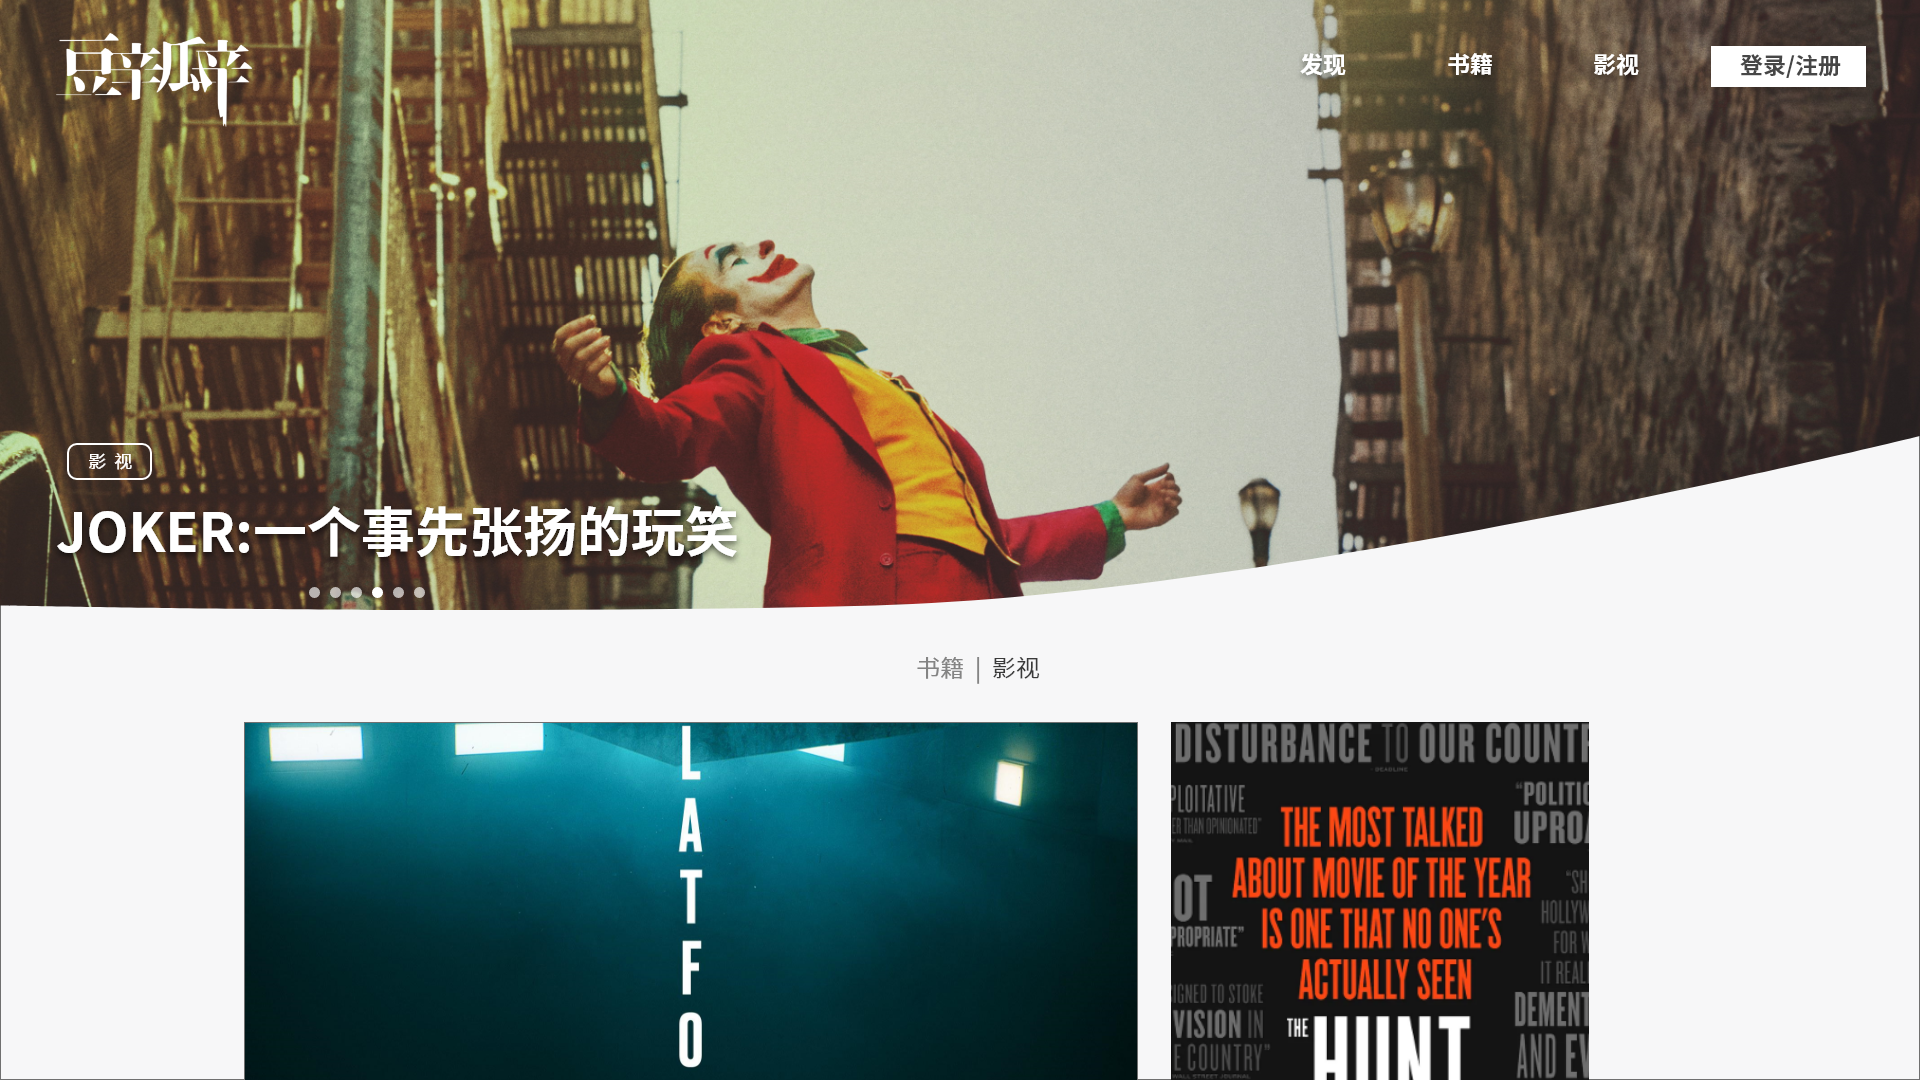
\includegraphics{D:/code/buaase-2020-chatplatform/docs/生成的LaTeX/pic/main.png}
\caption{}
\end{figure}

\textbf{包含功能模块:}

注册登录、浏览内容、检索内容。

\textbf{调用背景:}

网页的主页,热点内容的浏览页面,进入网页最先看到的页面。

\textbf{页面组成:}

透明导航栏,头版文章,热点推送内容。

\textbf{页面使用简介:}

进入网页最先看到的页面。用户和游客可以看到热点内容,可以进入书籍或者影视分类。

\hypertarget{header-n1302}{%
\paragraph{书籍、影视浏览页面}\label{header-n1302}}

\begin{figure}
\centering
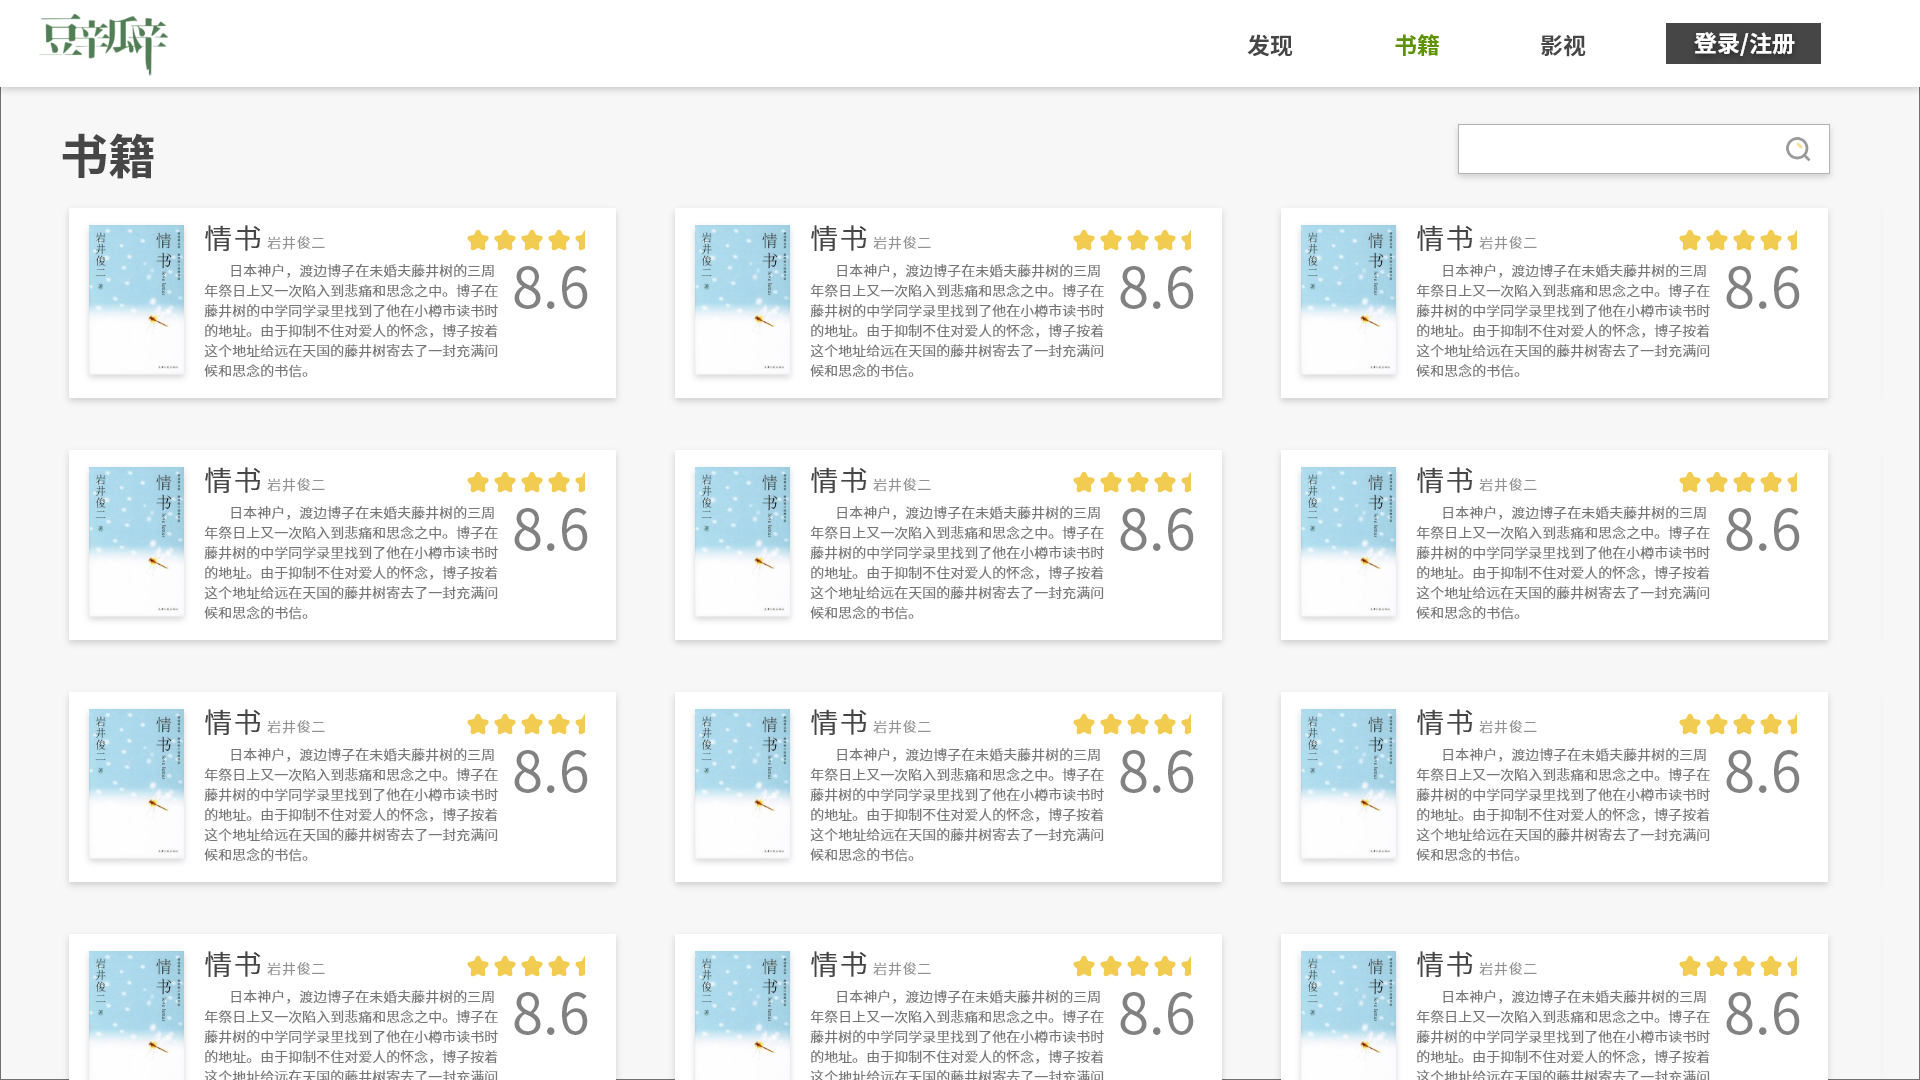
\includegraphics{D:/code/buaase-2020-chatplatform/docs/生成的LaTeX/pic/shuji.png}
\caption{}
\end{figure}

\textbf{包含功能模块:}

检索内容,浏览内容。

\textbf{调用背景:}

单击导航栏的书籍/影视标签后进入的页面。

\textbf{页面组成:}

导航栏,书籍内容。

\textbf{页面使用简介:}

在此页面,用户和游客可以看到书籍库总览,可以进入某一个书籍页面,也可以通过搜索查找到某一本书。

\hypertarget{header-n1312}{%
\paragraph{具体书籍、影视页面}\label{header-n1312}}

\begin{figure}
\centering
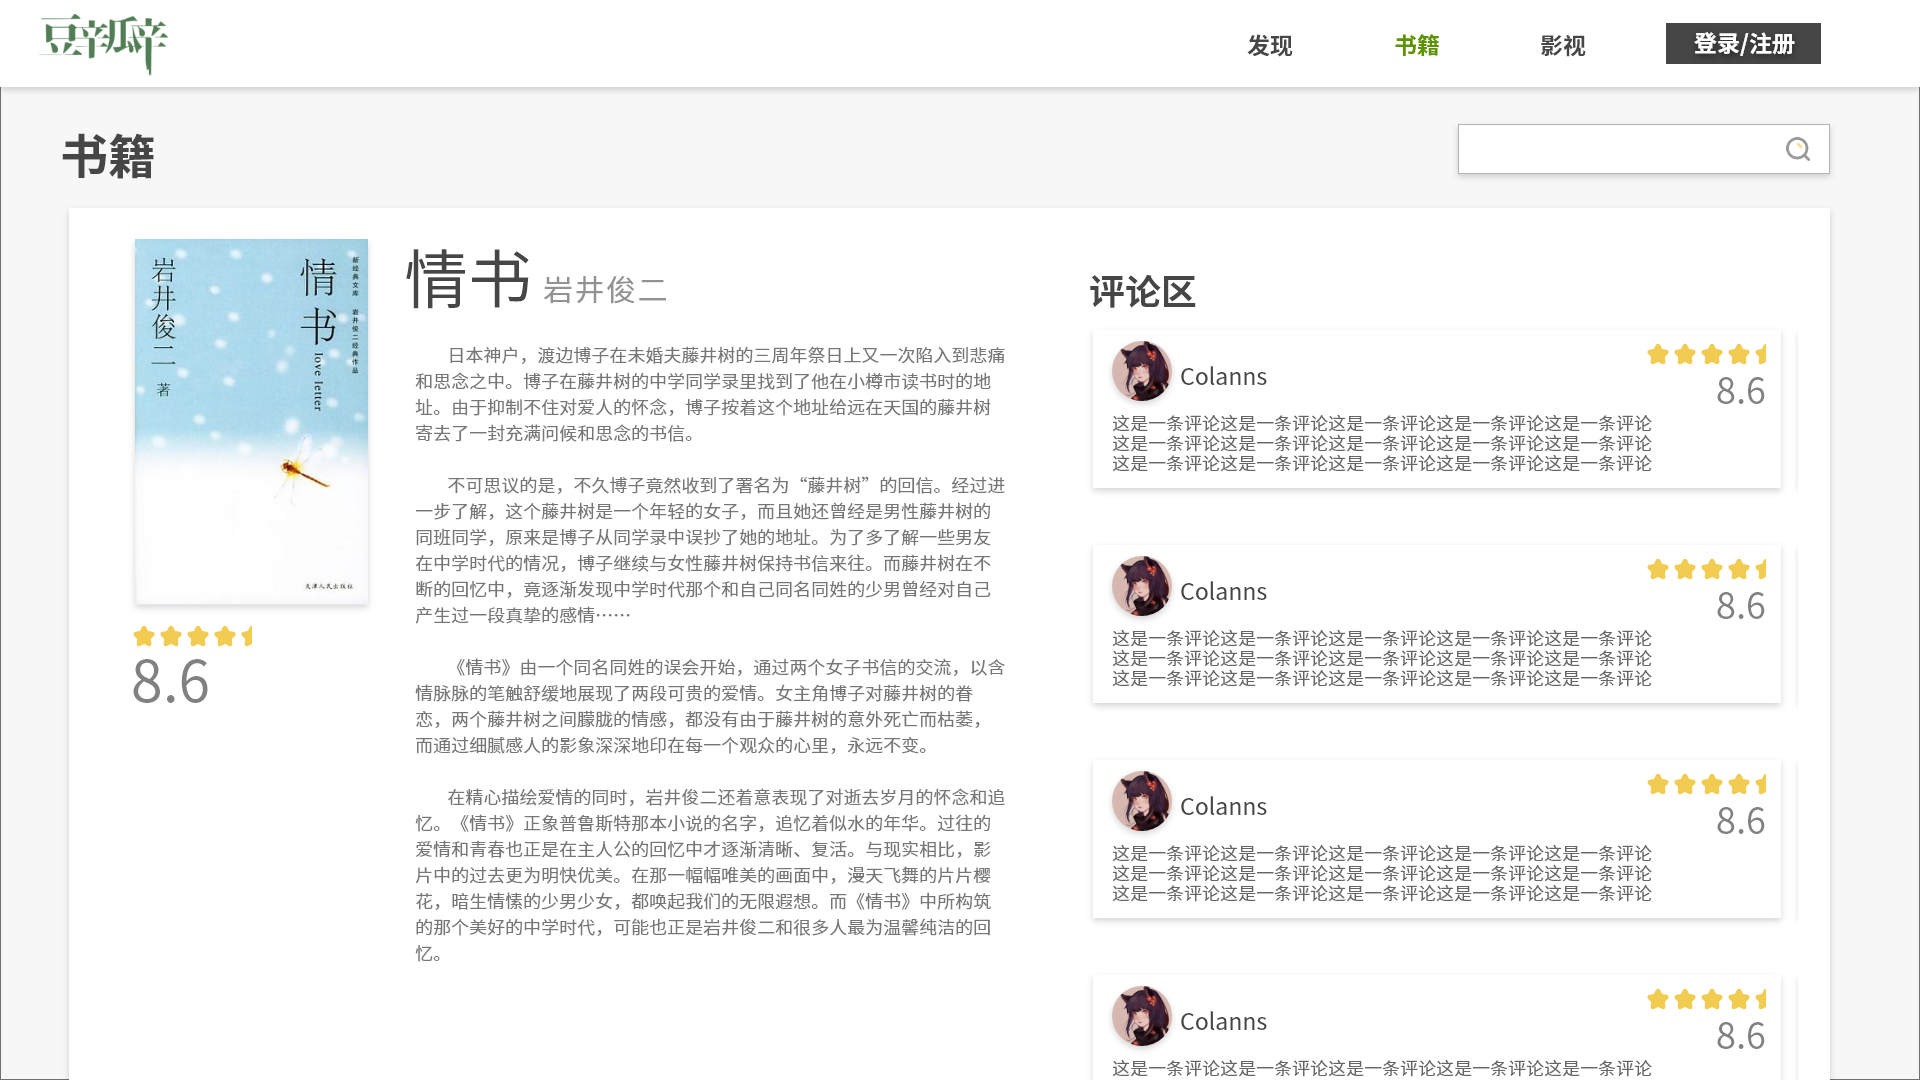
\includegraphics{D:/code/buaase-2020-chatplatform/docs/生成的LaTeX/pic/shujiju.png}
\caption{}
\end{figure}

\textbf{包含功能模块:}

评论书籍、评论影视、点赞评论、反对评论、举报评论、检索内容。

\textbf{调用背景:}

在浏览页面点击具体书籍即可进入此页面。

\textbf{页面组成:}

导航栏、书籍页面、搜索框、评论区。

\textbf{页面使用简介:}

在此页面下,用户可以对书籍进行评论,也可以对评论内容进行点赞、反对或者举报。

\hypertarget{header-n1322}{%
\paragraph{话题/小组页面}\label{header-n1322}}

\begin{figure}
\centering
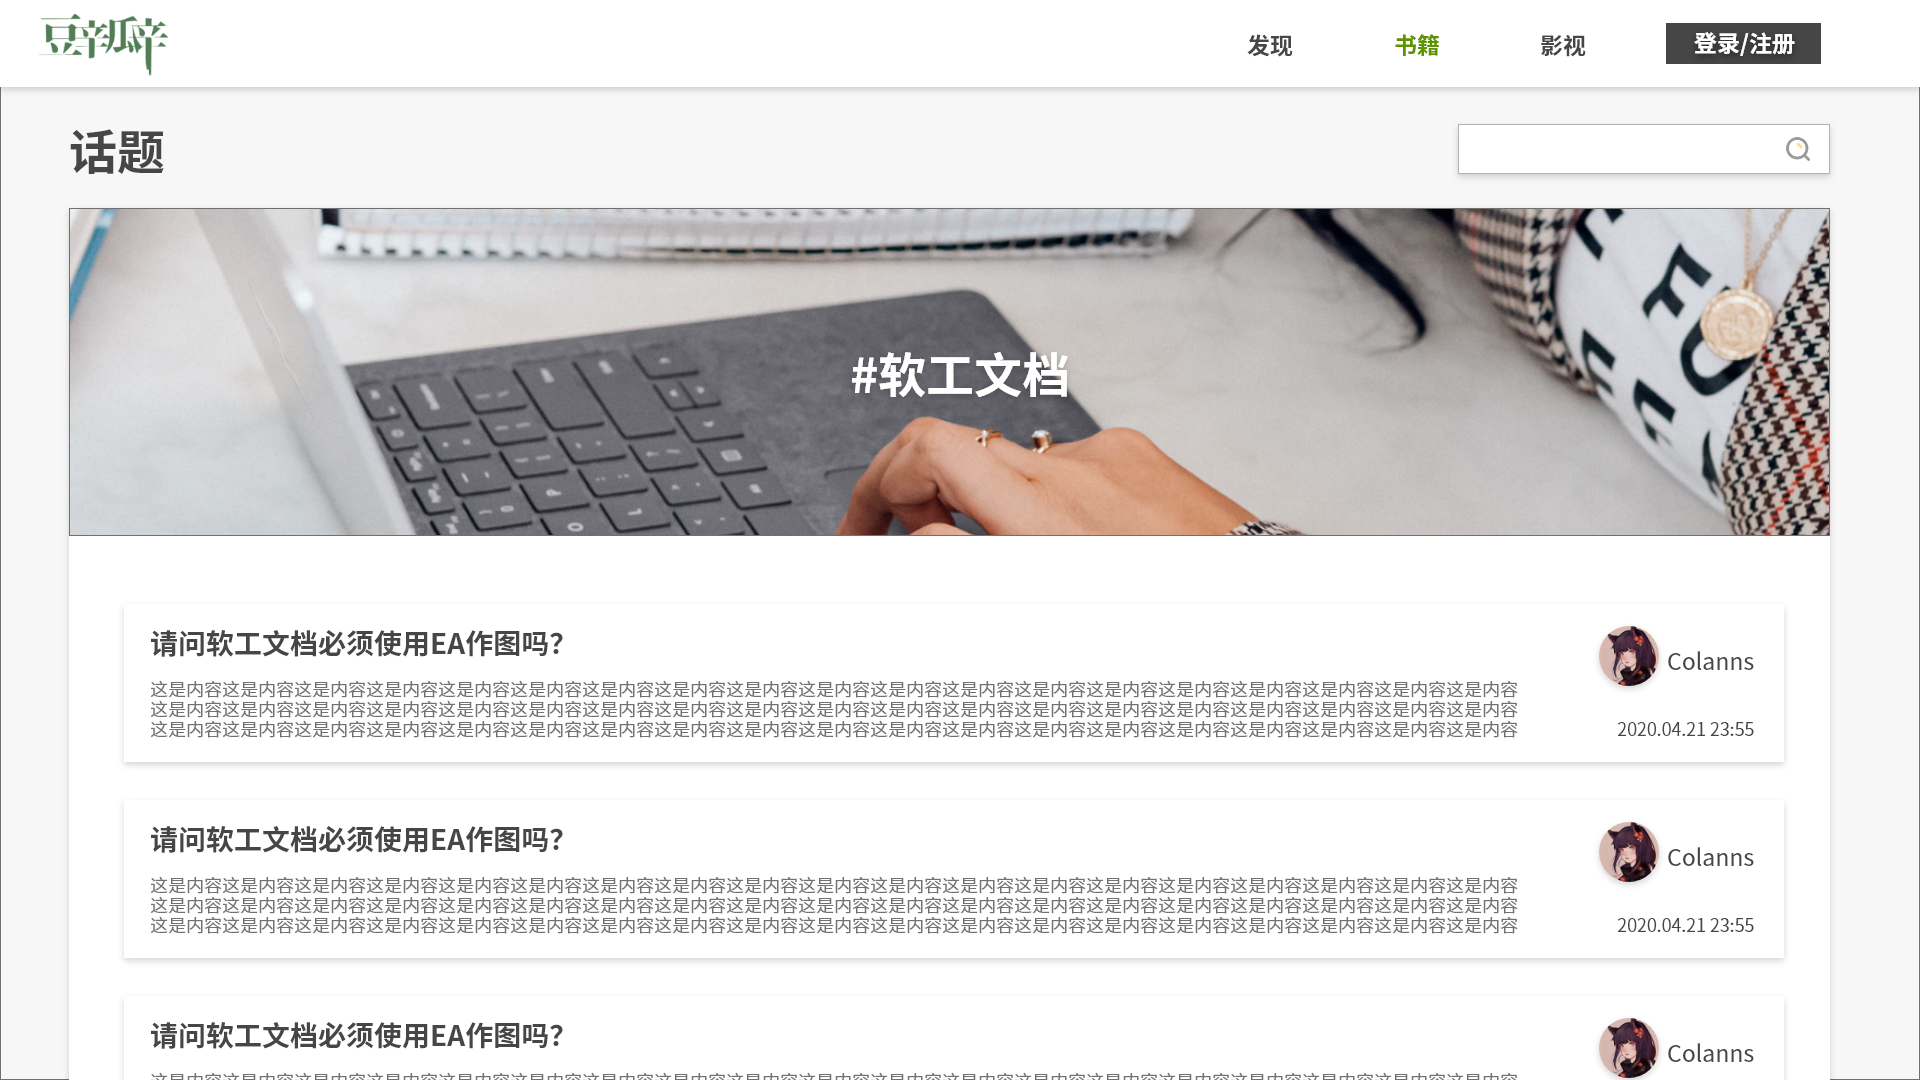
\includegraphics{D:/code/buaase-2020-chatplatform/docs/生成的LaTeX/pic/ht-xz.png}
\caption{}
\end{figure}

\textbf{包含功能模块:}

检索内容,浏览内容,参与话题,发表图文。

\textbf{调用背景:}

话题的具体页面,通过浏览话题页面(设计中)进入。

\textbf{页面组成:}

导航栏、书籍页面、搜索框、评论区。

\textbf{页面使用简介:}

用户可以在此页面参与讨论,发表图文或者检索内容。

\hypertarget{header-n1332}{%
\paragraph{注册登录页面}\label{header-n1332}}

\begin{figure}
\centering
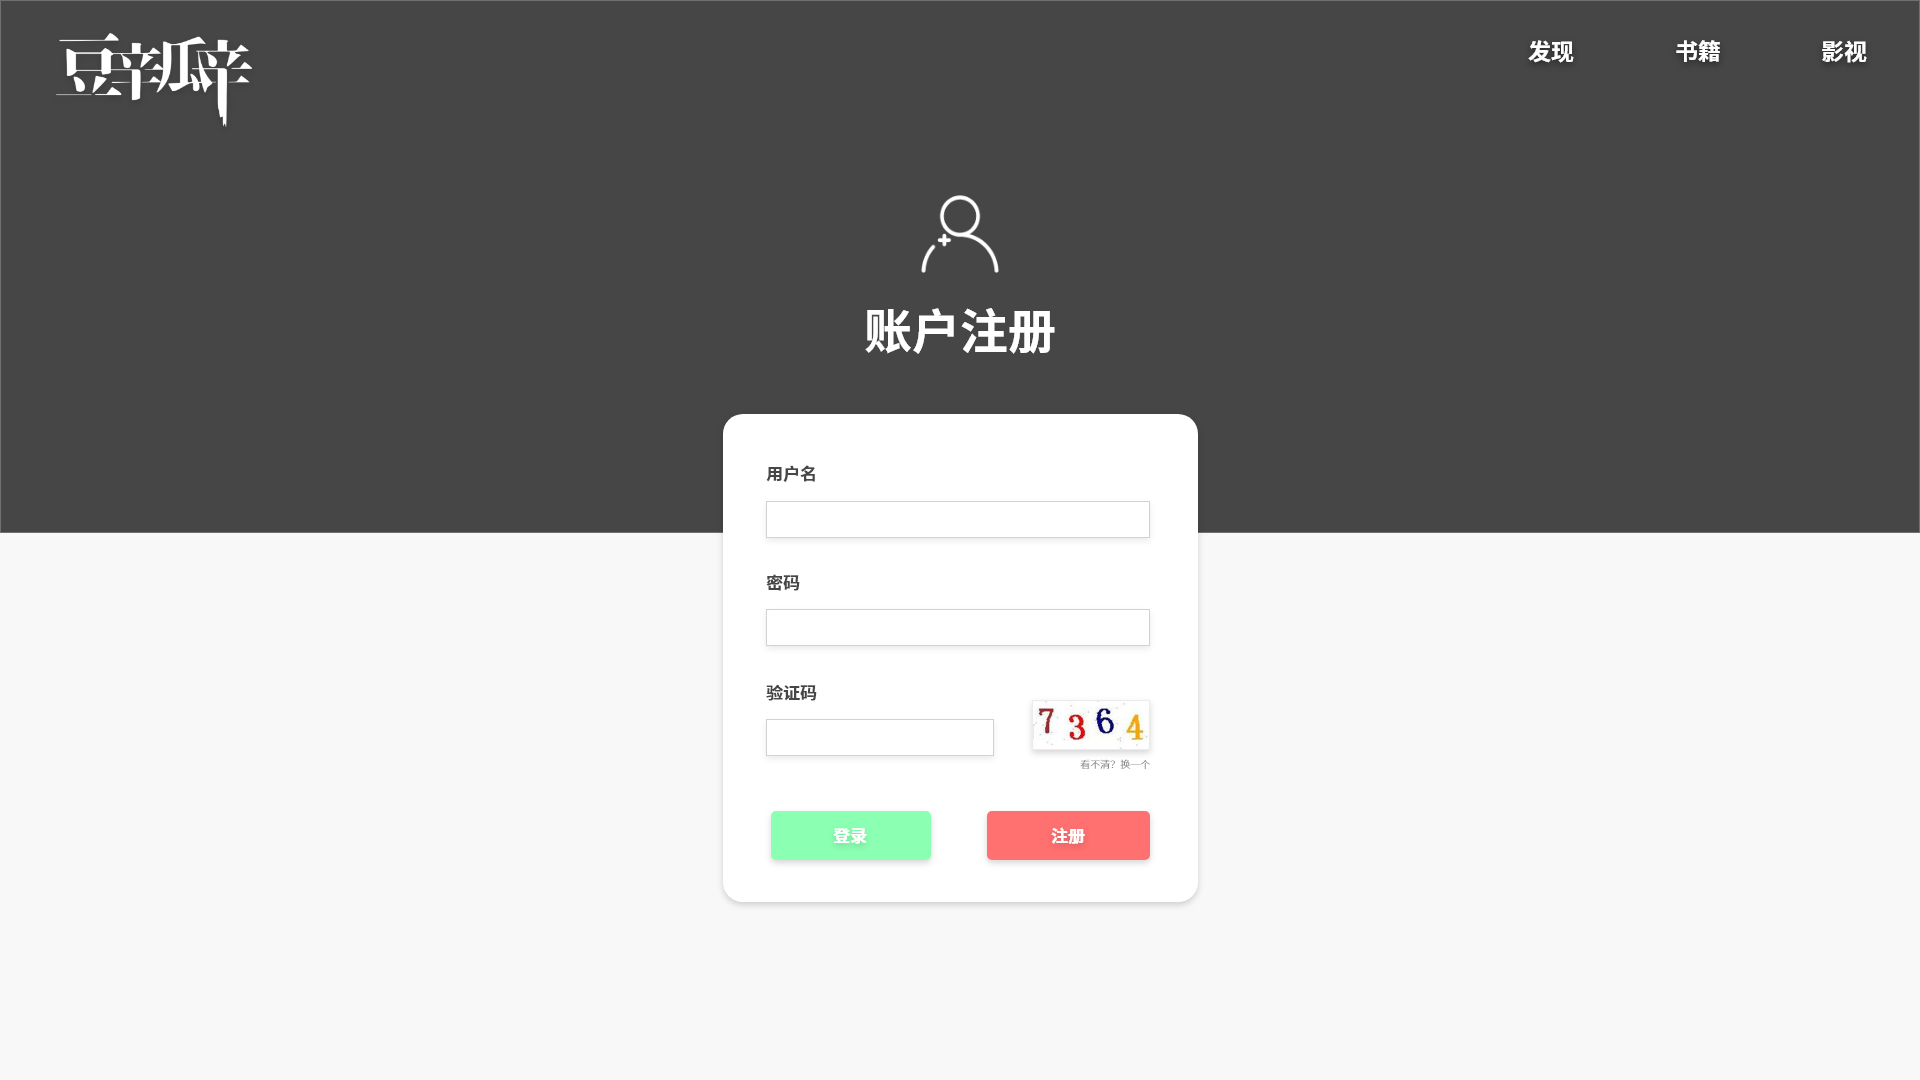
\includegraphics{D:/code/buaase-2020-chatplatform/docs/生成的LaTeX/pic/reglog.png}
\caption{}
\end{figure}

\textbf{包含功能模块:}

注册、登录、找回密码。

\textbf{调用背景:}

在任意页面点击右上角的注册/登录按钮。

\textbf{页面组成:}

导航栏、注册登录组件。

\textbf{页面使用简介:}

游客可以使用注册登录页面注册为用户或者登录为用户。

\hypertarget{header-n1342}{%
\paragraph{后台管理页面}\label{header-n1342}}

\begin{figure}
\centering
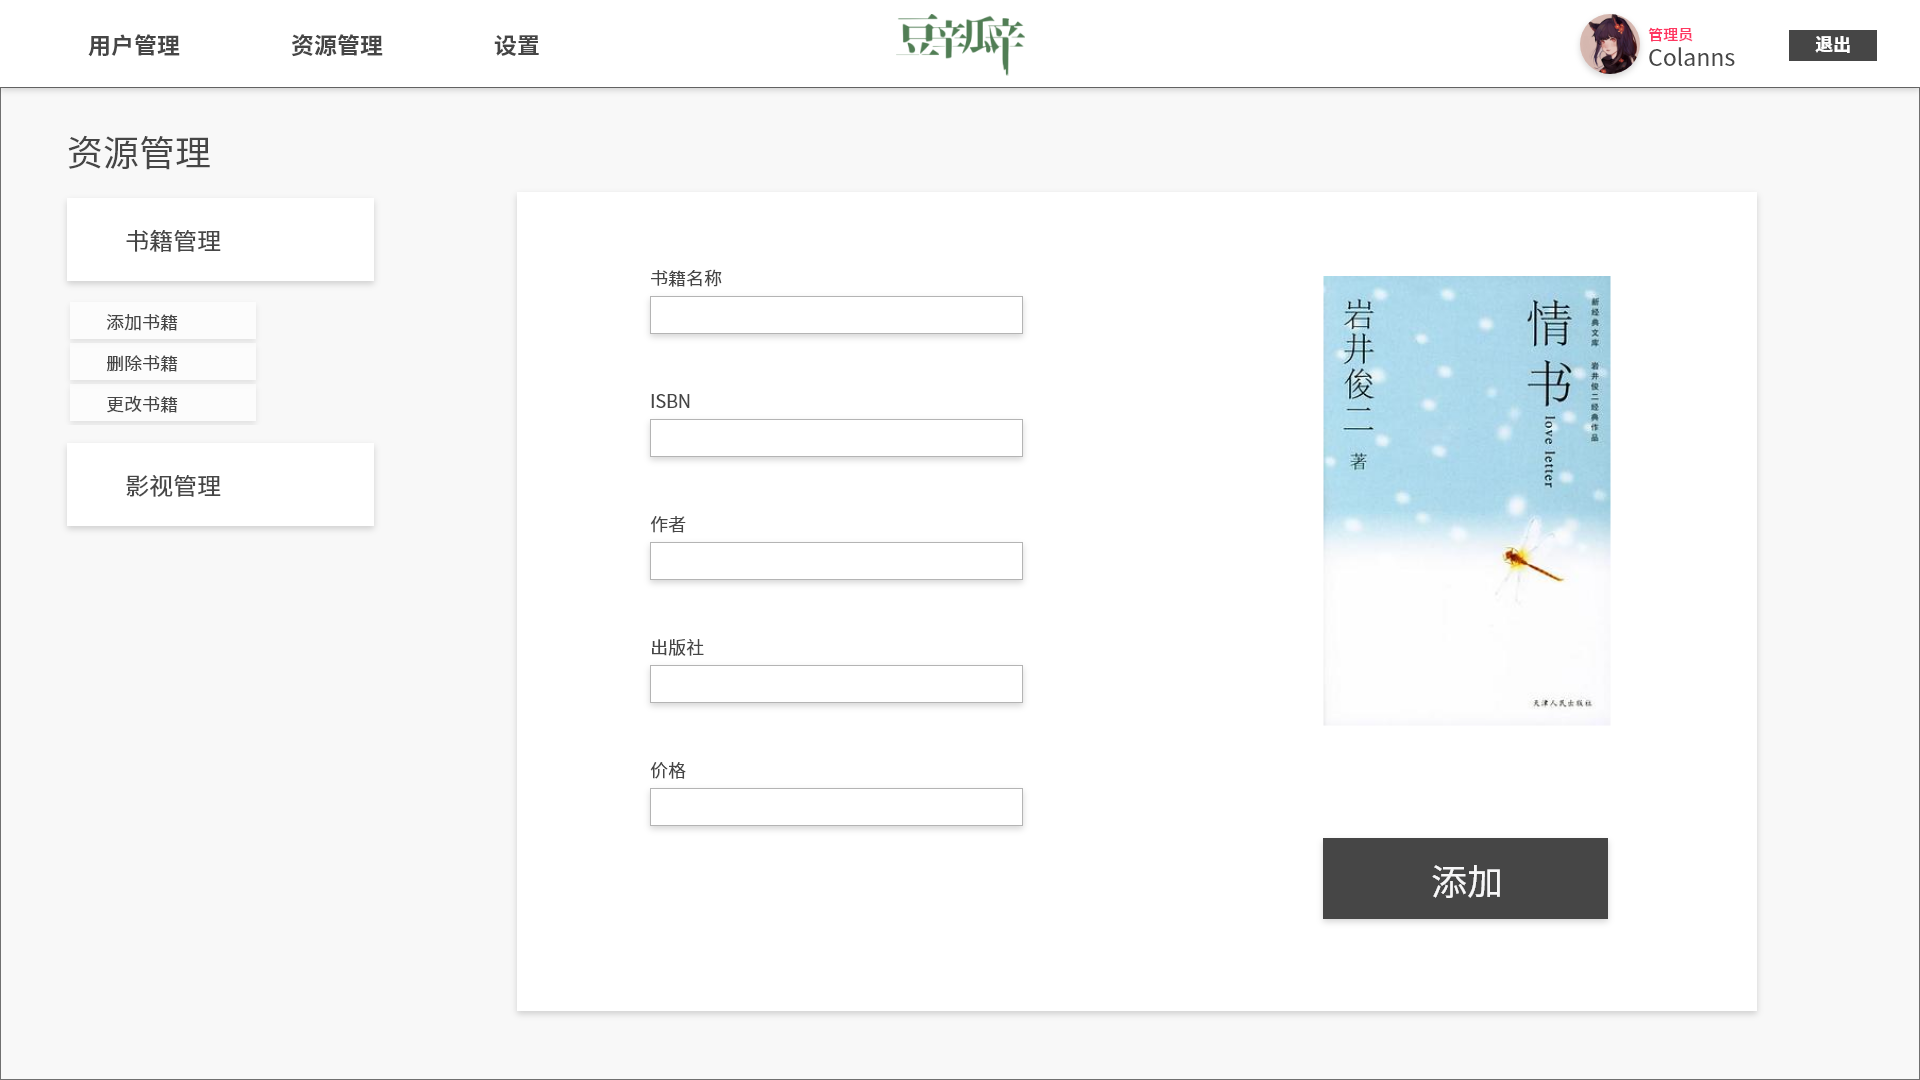
\includegraphics{D:/code/buaase-2020-chatplatform/docs/生成的LaTeX/pic/admin.png}
\caption{}
\end{figure}

\textbf{包含功能模块:}

查看个人信息、修改个人信息、删除用户、修改书籍内容。

\textbf{调用背景:}

管理员登录后可以进入此页面。

\textbf{页面组成:}

导航栏、管理组件。

\textbf{页面使用简介:}

管理员可以对书籍影视进行管理,也可以对用户进行管理操作。

\hypertarget{header-n1352}{%
\subsubsection{接口设计需求}\label{header-n1352}}

1.判断书籍影视作品的发布商是否有资格权限的接口

2.判断书籍影视作品的发布商提交的信息的接口

3.用户参与平台各种形式的交流反馈的接口

4.用户对平台相关数据进行检索的接口

5.用户进行相关管理审核工作的接口

6.用户进行登录注册的接口

\hypertarget{header-n1359}{%
\subsection{系统的其他需求}\label{header-n1359}}

\hypertarget{header-n1360}{%
\subsubsection{安全性}\label{header-n1360}}

平台能够保证用户相关信息的安全性,防止用户的个人隐私信息和资料泄露。同时需要能够维护平台的安全,保证平台上相关的书籍影视相关数据安全。同时,防止用户在书籍影视平台上进行各种违规非法的操作。

\hypertarget{header-n1362}{%
\subsubsection{可靠性}\label{header-n1362}}

同书籍影视平台能够保障平台上的相关书籍影视数据信息正确无误,确保书籍影视交流平台咨询内容详实,保证各个板块交流讨论的内容健康向上。

\hypertarget{header-n1364}{%
\subsubsection{灵活性}\label{header-n1364}}

系统平台的设计能够让用户在简洁直观的界面下进行操作和浏览,提高用户使用时的体验。

平台能够完成用户所需要的相关书籍影视作品的查找工作,以及能够完成对于书籍和影视作品的评论和反馈功能。

\hypertarget{header-n1367}{%
\subsection{系统的使用约束}\label{header-n1367}}

考虑到本系统仅为提供书籍影视资讯交流所用,所以暂时没有对使用进行什么特殊的约束,使用者可以假设以书籍影视平台用户的身份进行对系统的一些操作。

\end{document}
